\textnormal{The dataset has been generated by IBM and is based on a virtual world inhabited by individuals, companies, and banks. Individuals interact with other individuals and companies. Likewise, companies interact with other companies and with individuals. These interactions can take many forms, e.g. purchase of consumer goods and services, purchase orders for industrial supplies, payment of salaries, repayment of loans, and more. These financial transactions are generally conducted via banks, i.e. the payer and receiver both have accounts, with accounts taking multiple forms from checking to credit cards to bitcoin.
The data generator that created the data not only models illicit activity, but also tracks funds derived from illicit activity through arbitrarily many transactions. We use a higher illicit ratio (more laundering) for our project.\cite{IBMML}
The dataset (17 GB in size) contains 180 million records (100 bytes per record), 2.1 million distinct bank accounts, 15 distinct currencies
, and 7 distinct payment formats. The data was generated via the IBM simulation from August 1, 2022 to November 5, 2022.}\cite{Dataset}

\begin{figure}[htp]
    \centering
    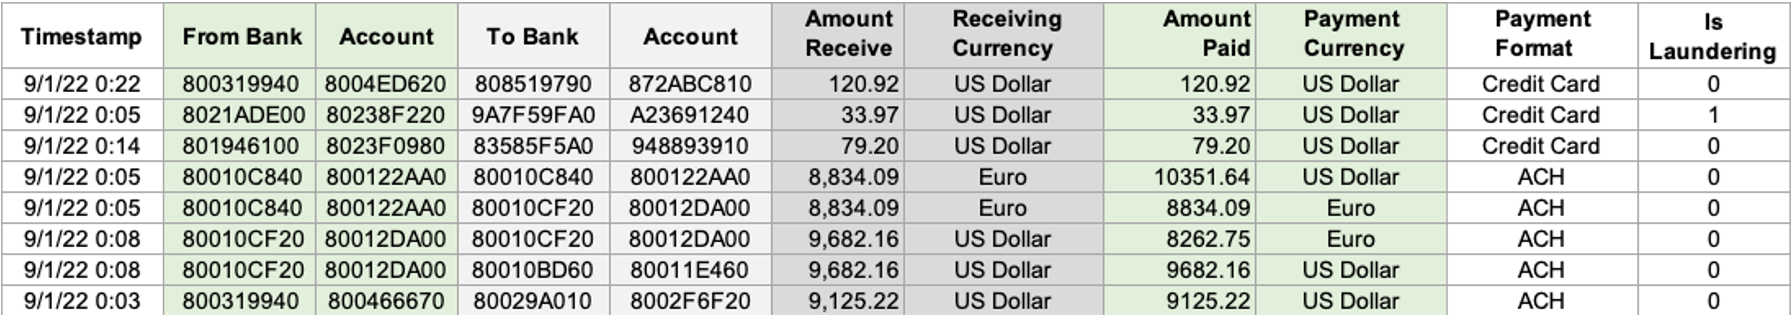
\includegraphics[width=8cm]{imgs/snapshot.png}
    \caption{Dataset Record Structure}
    \label{fig:DataFlowDiagram}
\end{figure}

\begin{figure}[htbp]
    \centering
    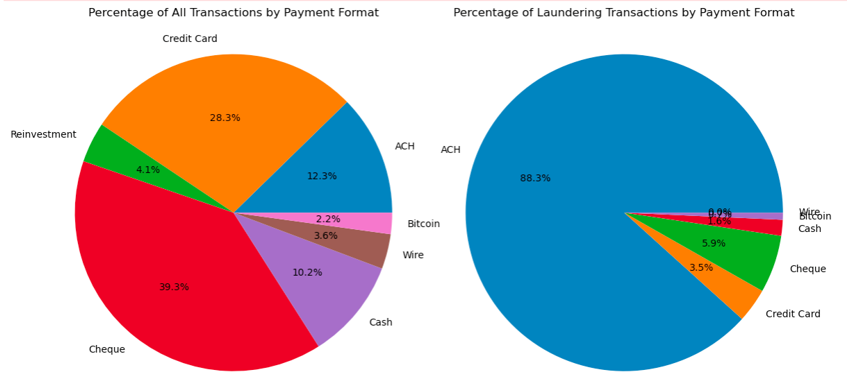
\includegraphics[width=7cm]{imgs/payment.png}
    \caption{Transactions in Payment Format}
    \label{fig:Data23}
\end{figure}

\begin{figure}[h]
    \centering
    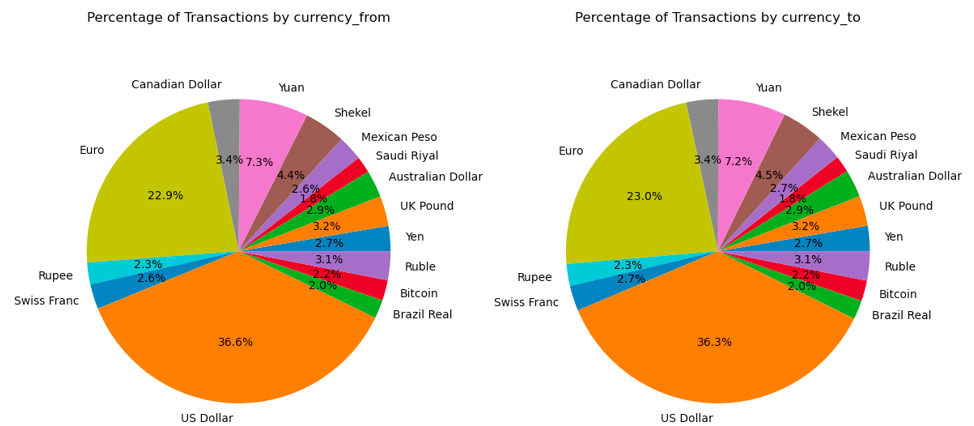
\includegraphics[width=8cm]{imgs/currency.png}
    \caption{Transactions in Currency Format}
    \label{fig:Diagram}
\end{figure}
